\section{Câu 10}
Thiết kế mạch dao động tạo sóng vuông đối xứng có chu kỳ 100KHz, chỉ dùng 1
OPAMP, các điện trở và tụ.

\begin{center}
\textbf{Bài giải}
\end{center}

Áp dụng kiến thức tạo xung bằng OPAMP sử dụng mạch với cả 2 hồi tiếp âm và dương như hình bên dưới.
\begin{figure}[H]
    \centering
    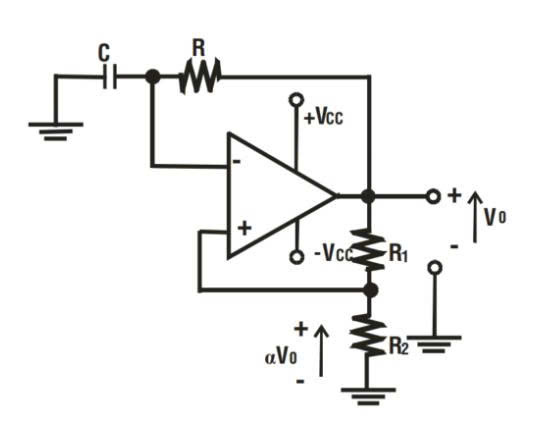
\includegraphics[scale=0.6]{image/StandardDesign_Cau10.png}
\end{figure}
Điều kiện đề bài cho là phải thiết kế mạch tạo sóng vuông đối xứng 100KHz nên ta có:
\begin{equation*}
    T = \dfrac{1}{f} = 10\mu s
\end{equation*}
\begin{equation*}
    T = T_1 + T_2 = 2T_1 = 2RC\ln\dfrac{1+\alpha}{1-\alpha}
\end{equation*}
\begin{equation*}
    \text{Với }  \alpha = \dfrac{R_2}{R_1 + R_2}
\end{equation*}
Từ dạng OPAMP trên ta chọn các thông số:
\begin{equation*}
    R_2 = 1k\Omega
\end{equation*}
\begin{equation*}
    R_3 = 1k\Omega
\end{equation*}
\begin{equation*}
    \alpha = \dfrac{1}{2}
\end{equation*}
\begin{equation*}
    \rightarrow T_1 = RC\ln 3
\end{equation*}
\begin{equation*}
    \rightarrow 10\mu s = 2RC\ln 3
\end{equation*}
\begin{equation*}
    \rightarrow RC = \dfrac{10\mu s}{2\ln 3} = 4.55\mu s
\end{equation*}
\begin{equation*}
    \text{Chọn } R_1 = 1k\Omega
\end{equation*}
\begin{equation*}
    \rightarrow C = 4.5nF
\end{equation*}

Chọn OPAMP LM7171AIM vì các thông số tham khảo được: \\
- Băng thông: 200MHz\\
- Slew Rate: 4100V/$\mu s$, phù hợp cho mạch so sánh và chuyển mạch nhanh\\
- Độ trễ ngõ ra so với ngõ vào thấp, phù hợp cho mạch tạo xung ổn định.\\
Mô phỏng mạch thu được kết quả:
\begin{figure}[H]
    \centering
    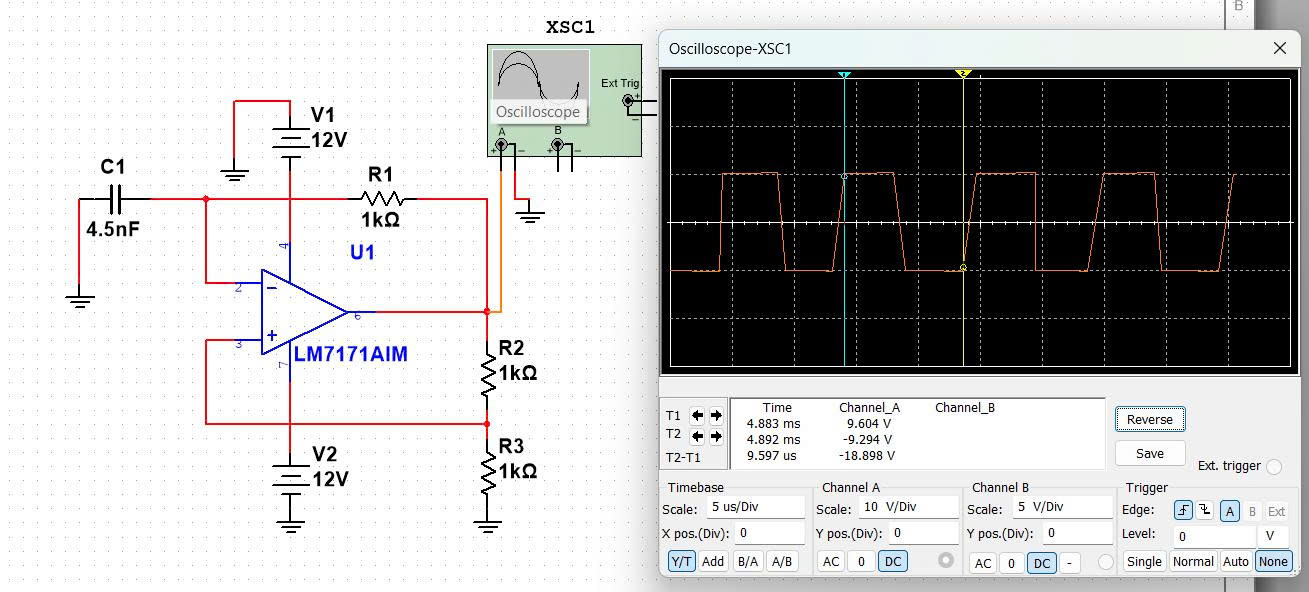
\includegraphics[scale=0.3]{image/C10.png}
\end{figure}